\documentclass[preprint,12pt]{elsarticle} %review, or preprint

\usepackage{amssymb}
\usepackage{graphics}
\usepackage{float}
\usepackage[normalem]{ulem}
\usepackage{color}
\usepackage{lscape}

\usepackage{mdframed} %For framing images


%Some code to display the units after the equation 
\usepackage{mathtools}
\makeatletter
\providecommand\add@text{}
\newcommand\tagaddtext[1]{%
  \gdef\add@text{#1\gdef\add@text{}}}% 
\renewcommand\tagform@[1]{%
  \maketag@@@{\llap{\add@text\quad}(\ignorespaces#1\unskip\@@italiccorr)}%
}
\makeatother



\graphicspath{{./Images/}}

\journal{Solar Energy Materials \& Solar Cells}

\begin{document}

\begin{frontmatter}

\title{Life Cycle Assessment of Dynamic Building Integrated Photovoltaics} 

\author[ita]{P. Jayathissa\corref{cor2} \tnoteref{t1}}
    \ead{jayathissa@arch.ethz.ch}
\address[ita]{Architecture and Building Systems, Institute of Technology in Architecture, Department of Architecture, ETH Zurich, Switzerland} 
% For whatever reason the affiliation needs to be defined after the authors. Otherwise the numbering gets messed up.

\author[ita]{M. Jansen\tnoteref{t1}}
    \ead{m.jansen@student.ethz.ch}

\author[baug]{N. Heeren}
    \ead{heeren@ifu.baug.ethz.ch}
\address[baug]{Ecological System Design, Institute of Environmental Engineering,\\ ETH Zurich, Switzerland}

\author[ita]{Z. Nagy}
	\ead{nagy@arch.ethz.ch}




\author[ita]{A. Schlueter \corref{cor1} }
    \ead{schlueter@arch.ethz.ch}

\tnotetext[t1]{Equally contributing first authors} 
\cortext[cor2]{Corresponding author}


\begin{abstract}
We assess the environmental impact of a dynamic, adaptive, building integrated photovoltaic (BIPV) systems. Such systems combine the benefits of adaptive shading with facade integrated solar tracking, thus reducing the building energy demand, and simultaneously generating electricity on-site. The inventory for the life cycle assessment (LCA) was acquired using production data, and Energy Plus simulations to calculate the building energy demand. The impact assessment was conducted according to ISO 14040 and ISO 14044 standards using the Eco-invent database and openLCA as an analysis tool. The embodied environmental impact of the dynamic BIPV solution is higher than a static alternative due to the added control system, electronics, actuators, and additional supporting structure, resulting in higher life cycle impacts. However when accounting for the systems multi functionality aspect, i.e. savings through adaptive shading to the building's heating, cooling and lighting loads, the embodied environmental impact can be offset, making the ASF an interesting alternative for BIPV. We also conduct a sensitivity analysis to investigate modifications to the actuator type, control system, and location and find that none of the investigated parameters overturn the key findings. The analysis ultimately enables us to provide design recommendations for future dynamic BIPV installations. 

\end{abstract}

\begin{keyword}
\sep Dynamic Photovoltaics \sep Life Cycle Analysis \sep Multi Functional Envelope \sep BIPV \sep Adaptive Shading
\end{keyword}

\end{frontmatter}

\section{Introduction}
\label{ch:introduction}
% !TEX root = main.tex

- In the last decades, building integrated photovoltaics (BIPV) have been adopted as part of the energy strategy towards 2050... \

(advantages of BIPV, potential of BIPV)\\
% Do we have a source for "have been adopted as part of the energy strategy towards 2050"?
%Yes - PJ

- The current developments of light-weight efficient thin film technologies have brought new design possibilities for architects in BIPV design... \

(Adaptive Building Envelopes, examples, Envelope is the barrier between the internal and external environment, Advantages, seamless coupling with solar tracking mechanics) \\

- One example of a multi functional facade that was recently released is the Adaptive Solar Facade.\\

- The aim of this paper is to analyse the life cycle emissions of an adaptive solar facade and provide comparisons with standard shading systems and static BIPV solutions.\\


\section{Methodology}
\label{ch:method}
% !TEX root = main.tex

In this section we detail the inventory, energy plus simulation methodology, important assumptions, and the LCA evaluation method. The assessment considers the environmental impacts of the production, operation, and disposal of an ASF. We assume a life time of 20 years based on the product warranty of the PV panels. \textcolor{cyan}{The Impact assessment is performed according to the ISO 14040 and ISO 14044, and is based off the IPCC methodology.}\\

\subsection{Embodied Life Cycle Inventory}

The inventory data was obtained from technical drawings, research papers describing the technology, and expert judggement. The Ecoinvent v3.1 database is used as the main LCA database \cite{frischknecht2005ecoinvent}. The cut-off approach is used for the allocation of recycling and landfill disposal. This means that recycling does not generate any credit for the product and resulting benefits are not taken into account. Furthermore the use of recycled products do not bear the burden of processes higher up the chain.\\

The mechanical components of the ASF can be broken into four parts: a PV panel, actuator, cantilever, and a cable net supporting structure. The PV panel, actuator and cantilever combine to form a dynamic PV module, which is then mounted on a cable net supporting structure. An exploded view of these components can be seen in Figure \ref{fig:explodedView}. There are also additional electronics which exists off the facade in a separate control box. Theses five components along with the assembly, are the main product systems in the manufacture of the ASF as seen in Figure \ref{fig:BOS}. 

%\textcolor{magenta}{\textit{\\It is absolutely necessary that we describe the system boundary (what is included and what not (e.g. transport) and why) and also the functional unit! Were all life phases properly described? What happens in the maintenance, disposal phase? Will we have an annex? If so, we should give the ecoinvent inventories there.}}


% \begin{figure}[H]
% \begin{center}
% 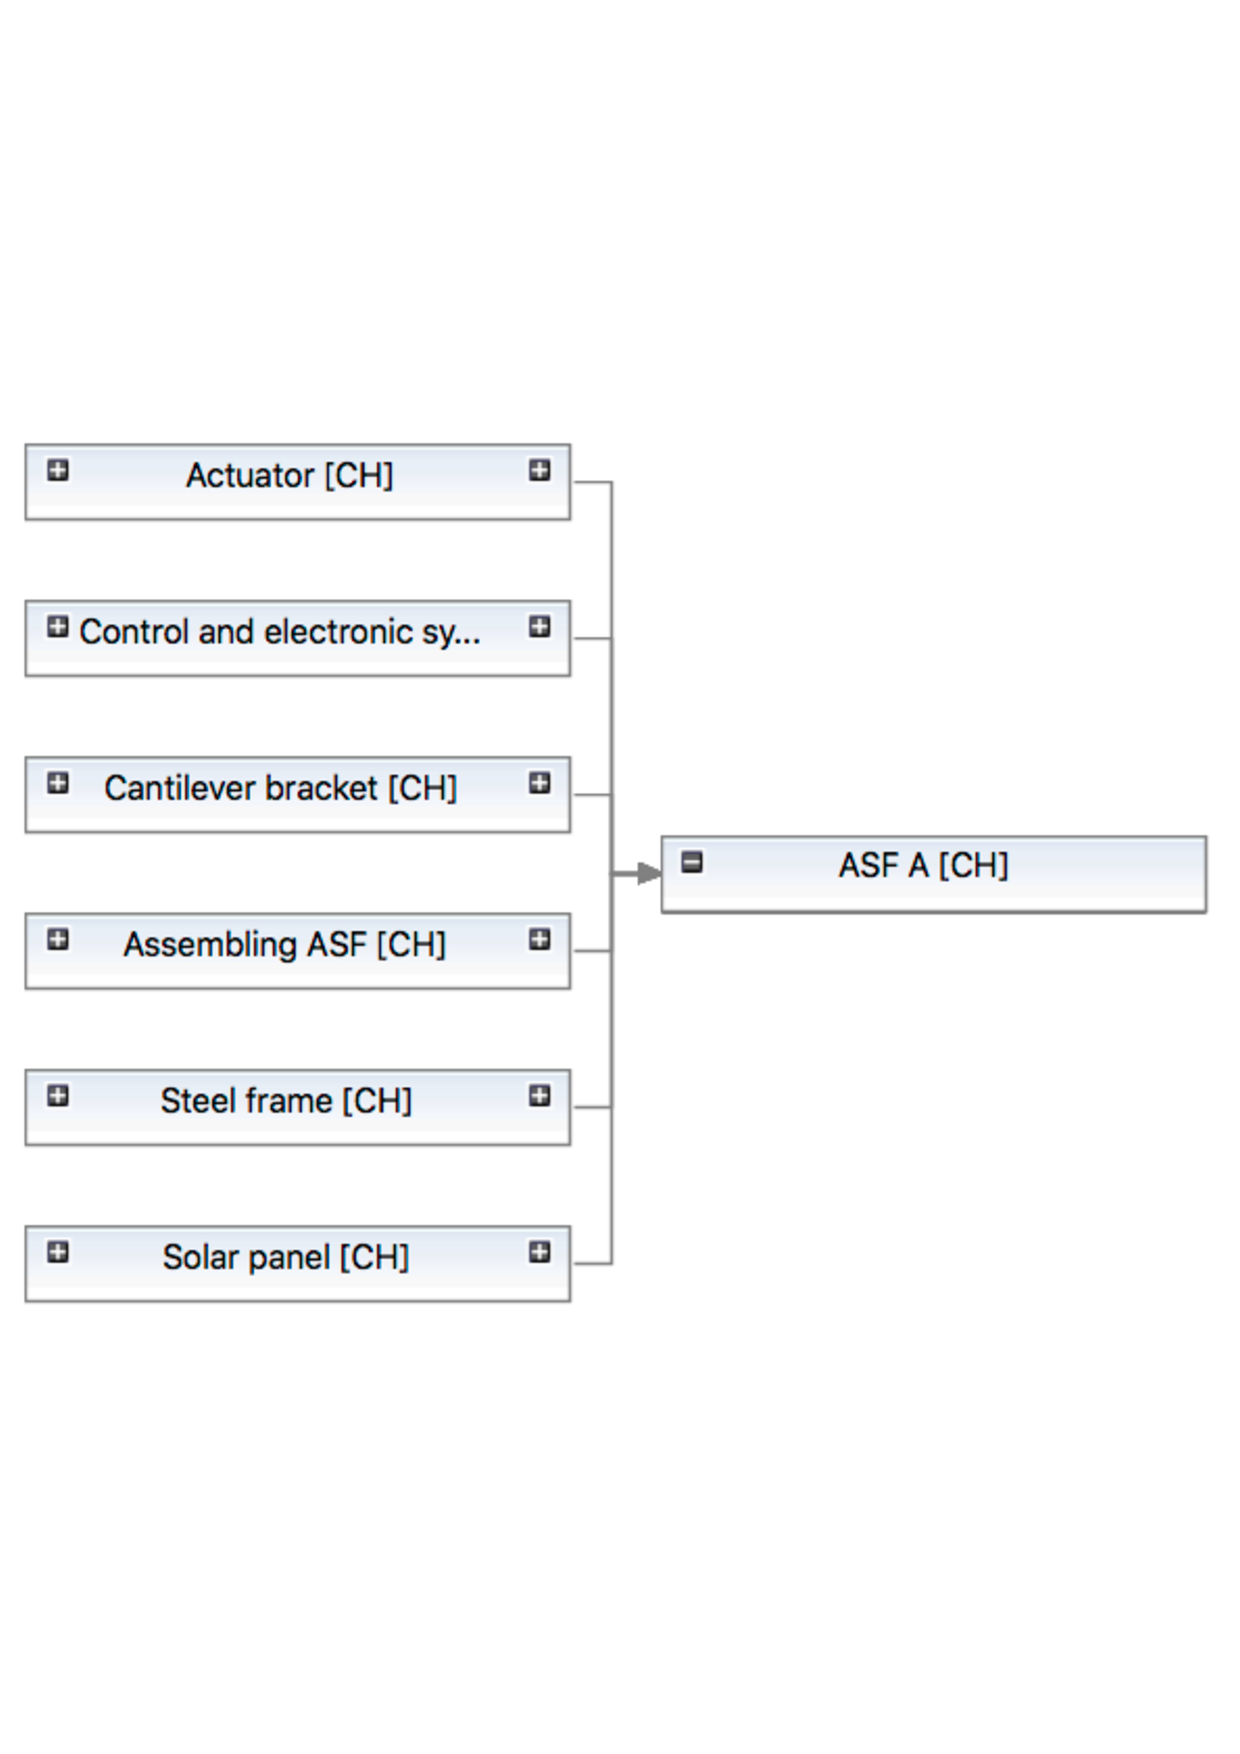
\includegraphics[width=8cm, trim= 0cm 0cm 0cm 0cm,clip]{ASFSubsystems.pdf}
% \caption{Breakdown of the ASF into six sub-product systems (Note change Steel frame to Suporting Structure, and Assembling ASF to Assembly. Also redraw this chart so it matches the subsubsections below)}
% \label{fig:subsystem}
% \end{center}
% \end{figure}

\begin{figure}[H]
\begin{center}
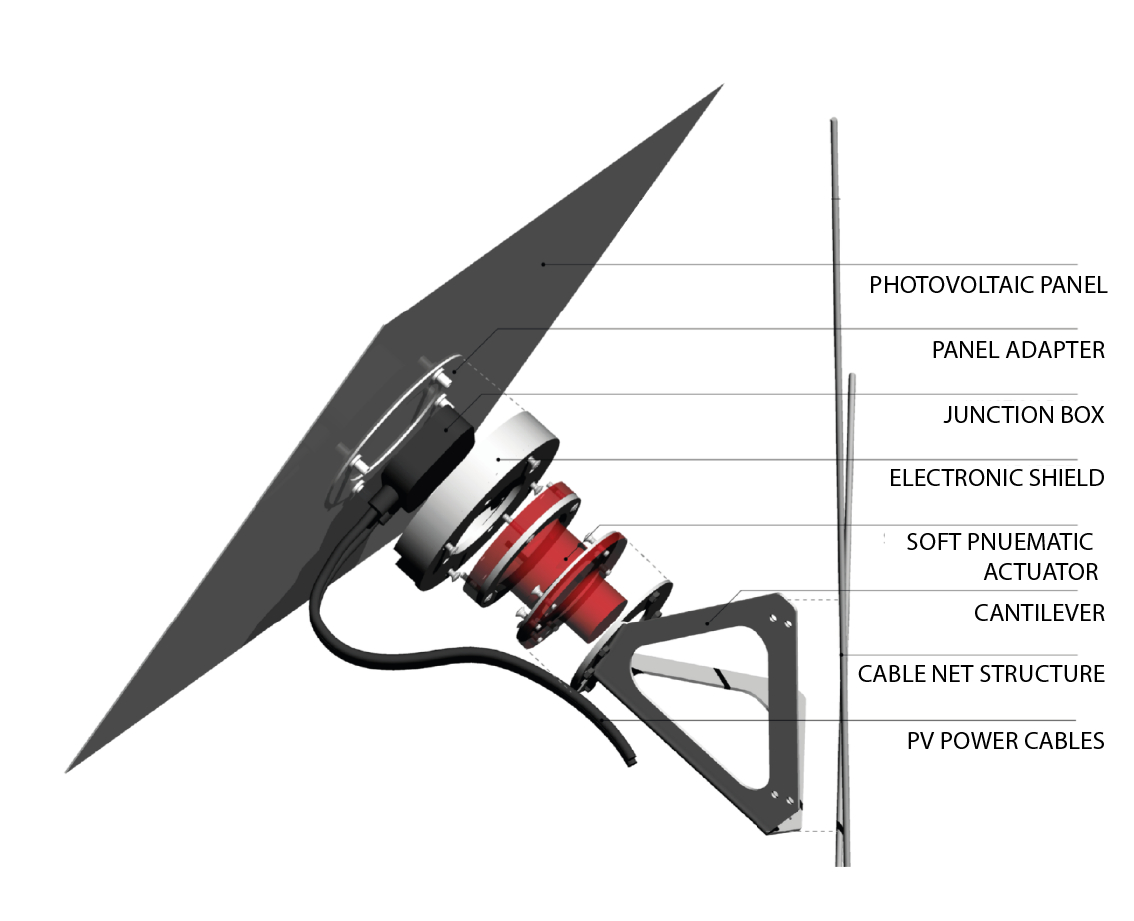
\includegraphics[width=8cm, trim= 0cm 0cm 0cm 0cm,clip]{explodedASFV2.png}
\caption{Exploded view of an ASF module mounted on a cable net supporting structure}
\label{fig:explodedView}
\end{center}
\end{figure}

\begin{figure}[ht]
\begin{center}
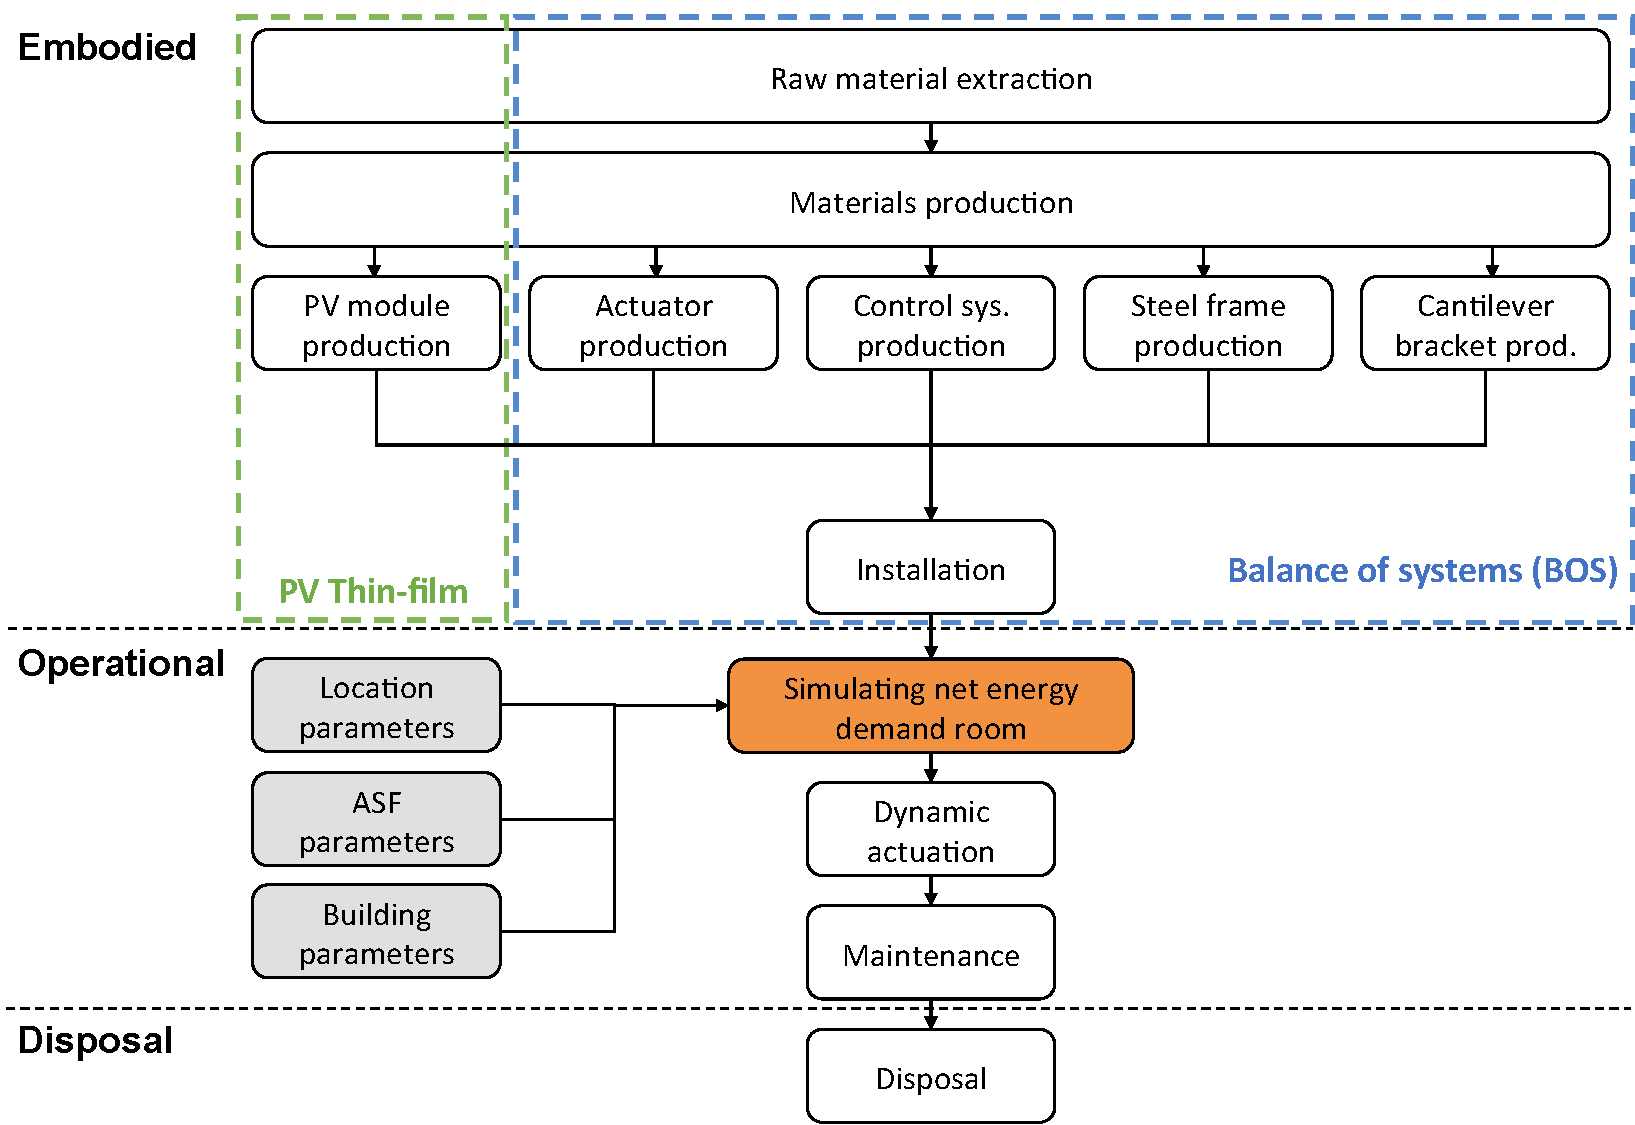
\includegraphics[width=14cm, trim= 0cm 0cm 0cm 0cm,clip]{BOS.pdf}
\caption{Breakdown of the ASF into five embodied product components and installation costs, operational costs, and disposal}

\label{fig:BOS}
\end{center}
\end{figure}
\textcolor{magenta}{\textit{(May Move the text to an Appendix and just keep the inventories)}}
\begin{description}

\item[PV Panel] \hfill\\
Weight is the primary restriction when selecting a PV panel. Any technology that requires glass encapsulation or a heavy substructure can therefore not be used. This limits us to CIGS and amorphous silicon panels.\\

CIGS PV panels were selected as the thin film panel of choice due to its high efficiency, low cost, and ability to be deposited on a polymer or aluminium substrate \cite{chirilua2011highly}. 

%A less efficient thin film amorphous silicon panel could also be used and will also be discussed in this analysis.\\

\textcolor{magenta}{\textit{(Not sure if it makes sense to provide the entire inventory here. If so, we would probably also need to give expected lifetimes, etc.)}}

% \begin{table}[H]
% \centering
% \begin{tabular}{lll}
% Panel Type  & SMQ    & ${\mathrm{\eta}}$  \\
% \hline
% CIGS 				& 0.7036 ${\mathrm{m^2_{panel}/m^2}}$ & \% \\
% a-Si				 	& 0.7036 ${\mathrm{m^2_{panel}/m^2}}$ & YY\%    \\
% Aluminum sheet 		& x ${\mathrm{kg/m^2}}$
% \end{tabular}
% \caption{Possible PV technologies for an ASF [Ref required]}
% \label{tab:PV}
% \end{table}

\begin{table}[H]
\centering
\begin{tabular}{ll}
\hline
Material description & SMQ \\ \hline
CIGS PV film       	 & 0.569 ${\mathrm{m^2_{PV}/m^2_{facade}}}$\\
Aluminum sheet 	 & 1.593 ${\mathrm{kg/m^2_{facade}}}$\\
Chromium steel panel adapter  & 1.422 ${\mathrm{kg/m^2_{facade}}}$\\
Polyethylene for junction box & 0.036 ${\mathrm{kg/m^2_{facade}}}$\\
Diode, glass for junction box & 0.011 ${\mathrm{kg/m^2_{facade}}}$\\
\hline
\end{tabular}
\caption{Inventory of the top five input flows to the PV manufacturing process [ref required]}
\label{tab:PVinv}
\end{table}

\item[Actuator] \hfill \\
Traditionally photovoltaic actuation is done through the use of servo motors. Servo motors however become a limiting factor for adaptive facades due to their high upfront costs, and instability in heavy winds. Soft robotic actuators on the other hand are cheaper and more resilient to harsh environmental conditions\cite{Svetozarevic2014a}. The soft robotic actuators however are still in development and have a life time of five years. They will therefore require three rounds of maintenance during the lifetime of the ASF.
For the purpose of this analysis we will analyse both servo motors and soft robotic actuators. 

\begin{table}[H]
\centering
\begin{tabular}{ll}
\hline
Material description & SMQ \\ \hline
Chromium steel rings	 & 1.0665 ${\mathrm{kg/m^2_{facade}}}$ \\
Electronics, for control, 2-2way valves  & 0.0130  ${\mathrm{kg/m^2_{facade}}}$\\
Silicone chambers & 0.8887 ${\mathrm{kg/m^2_{facade}}}$\\
Polyurethane tubes &0.0933 ${\mathrm{kg/m^2_{facade}}}$\\
Air compressor, screw type, 0.75kW & 1.7281 ${\mathrm{kg/m^2_{facade}}}$\\
\hline
\end{tabular}
\caption{Inventory of four main input flows to the actuator manufacturing process [ref required]}
\label{tab:ActuatorInv}
\end{table}

\item[Cantilever] \hfill \\
The cantilever is a steel connection point between the PV panel and the supporting structure.\\

\begin{table}[H]
\centering
\begin{tabular}{ll}
\hline
Material description & SMQ \\ \hline
Chromium steel bracket	 & 1.4220 ${\mathrm{kg/m^2_{facade}}}$ \\
Chromium steel fixing clamp  & 0.0284 ${\mathrm{kg/m^2_{facade}}}$\\
\hline
\end{tabular}
\caption{Inventory of main input flows to the Cantilever manufacturing process [ref required]}
\label{tab:CantileverInv}
\end{table}

\item[Supporting Structure] \hfill \\
The supporting structure is the connection point between the array of photovoltaic modules and the building itself. Many different designs are possible, however we will base our analysis of an adaptive solar facade that has already been constructed \cite{nagy2015frontiers}. This design consists of a steel cable-net that spans a steel supporting frame. The steel frame is then mounted on the building facade.\\

\begin{table}[H]
\centering
\begin{tabular}{ll}
\hline
Material description & SMQ \\ \hline
Chromium steel frame & 6.9928 ${\mathrm{kg/m^2_{facade}}}$ \\
Chromium steel swaged external thread  &0.2897 ${\mathrm{kg/m^2_{facade}}}$\\
Chromium steel wire rope WC  & 0.1593 ${\mathrm{kg/m^2_{facade}}}$\\
\hline
\end{tabular}
\caption{Inventory of the four main input flows to the manufacturing process of the Supporting Structure[ref required]}
\label{tab:StructureInv}
\end{table}

\item[Control System and Electronics] \hfill \\
The control system is required for the actuation of panels and the regulation of photovoltaic electricity production.\\

\begin{table}[H]
\centering
\begin{tabular}{ll}
\hline
Material description & SMQ \\ \hline
Inverter 1.25kW	 & 0.6090 ${\mathrm{kg/m^2_{facade}}}$ \\
PV cable  & 3.1995 ${\mathrm{kg/m^2_{facade}}}$\\
Electronics control\footnote{c-Rio,8-slot, integrated 667Mhz}& 0.0419 ${\mathrm{kg/m^2_{facade}}}$\\
Electronics control\footnote{NI9476 32ch DO with cables and connectors}& 0.0097${\mathrm{kg/m^2_{facade}}}$\\
\hline
\end{tabular}
\caption{Inventory of the four main input flows to the manufacturing process of the Control System[ref required]}
\label{tab:ControlInv}
\end{table}

\item[Assembly] \hfill \\
There are many assembly options available. From past experience, an installation of an equivalent ASF required a hydraulic hoist which was in operation for eight hours \cite{jayathissa2015abs}. \\

\begin{table}[H]
\centering
\begin{tabular}{ll}
\hline
Material description & SMQ \\ \hline
Hoist, diesel  ${<}$18.64kW, idling & 0.5267 ${\mathrm{h/m^2_{facade}}}$ \\
\hline
\end{tabular}
\caption{Inventory of main input flows to the Assembly Process[ref required]}
\label{tab:AssemblyInv}
\end{table}

\end{description}

\subsection{Operational Life Cycle Inventory}
\label{ch:Meth:Opp}

The operational inventory are categorised as 1) energy consumption of an office room 2) electricity consumption through dynamic actuation, and 3) maintenance.

\begin{description}


\item[Building Energy Consumption: ] \hfill\\
An adaptive shading system, when mounted over a glazed facade, has an impact on the energy consumption of the building as described in Section \ref{ch:introduction}. More specifically, it has an impact on the heating cooling and lighting loads. Previously conducted simulations compared three scenarios: 1) facade with no shading, 2) a facade with a static shading system angled at 45$^{\circ}$ to the horizontal axis, and 3) an adaptive solar facade \cite{jayathissa2015abs}.\\

The simulation was conducted on a south facing office room. The room 7.0 meters in length, 4.9 meters wide and 3.1 meters high was modeled using Rhinoceros 3D CAD Package \cite{Rhino}. Grasshopper \cite{grasshopper} was used to model the orientation of each photovoltaic panel. The geometrical input is imported to Energy Plus \cite{energyplus} though the DIVA \cite{DIVA} interface. A single zone thermal analysis was conducted for each possible geometrical configuration of the ASF for each hour of the year. The results were then post processed in MATLAB.\\

The simulations show a total energy saving of 25\% compared to louvers at 45$^\circ$ and 56\% compared to a case with no facade shading \cite{jayathissa2015abs}. These results are sumarised in Figure \ref{fig:operational}. \\


\begin{figure}[H]
\begin{center}
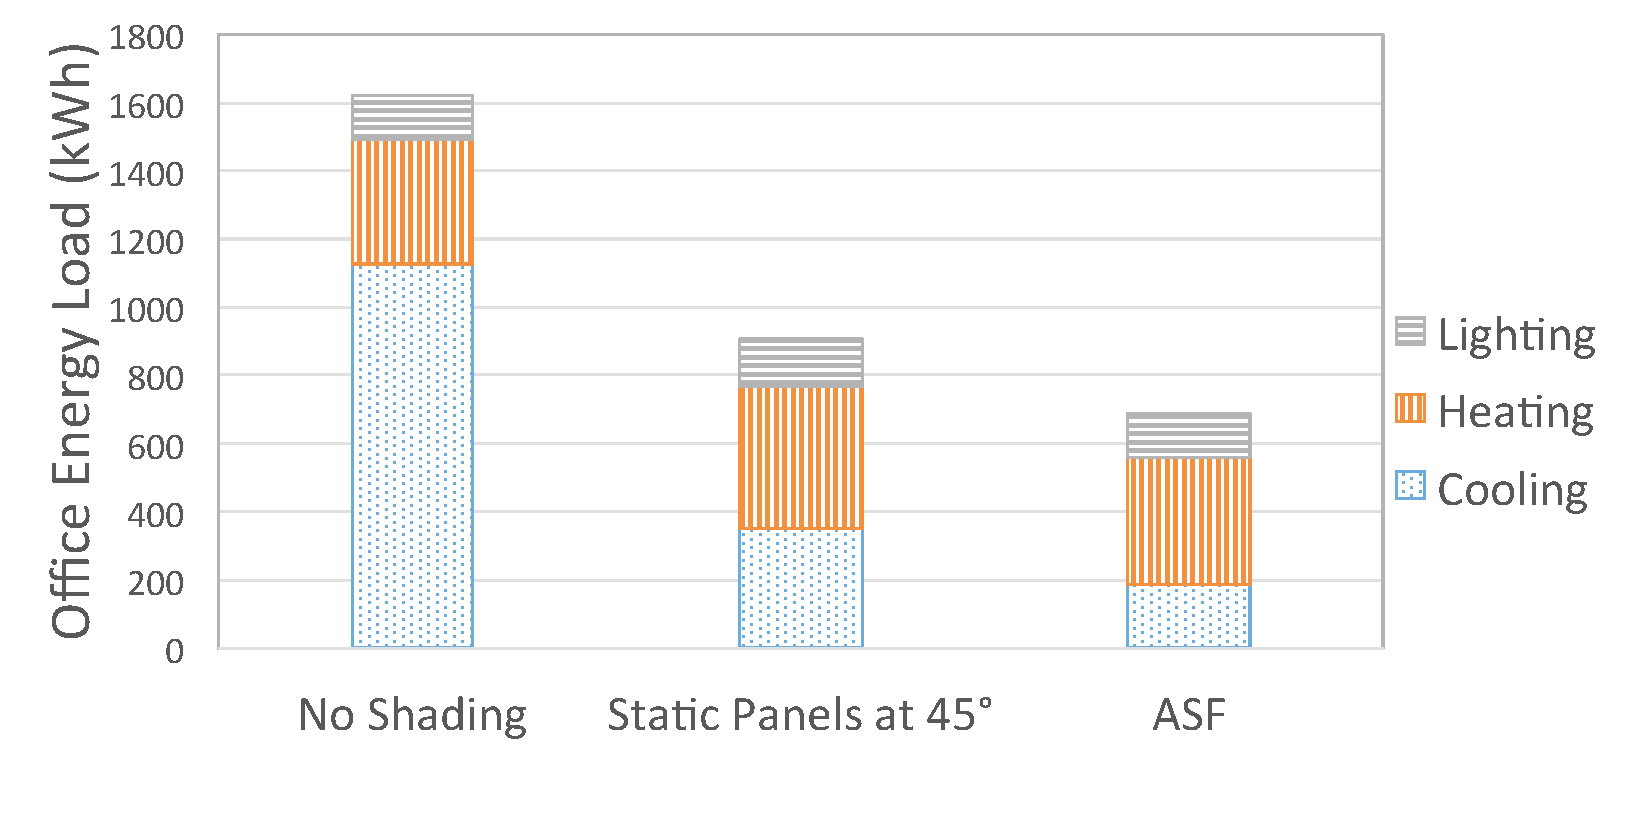
\includegraphics[width=10cm, trim= 0cm 0cm 0cm 0cm,clip]{buildingenergy.pdf}
\caption{Breakdown of operational energy consumption for a system with a) no shading, b) with louvers at 45$^\circ$ and c) with an ASF -- not including onsite electricity production.}
\label{fig:operational}
\end{center}
\end{figure}

% ASF, when mounted over a glazed surface has an impact on the energy consumption of the office space behind the facade. In particular 
% An adaptive shading system reduce the electrical consumption of a building through reductions in heating, cooling and lighting \cite{jayathissa2015abs}. \textcolor{magenta}{\textit{I'd be more verbose. How does it affect energy demand? A "saving" is always relative - so it should probably refer to a base case.}}
% These electrical savings can be translated into GWP savings based on the emission factor of the European Network of Transmission System Operators for Electricity (ENTSO-E) electricity mix (462.1gCO2/kWh)\cite{itten2012life}.\\



\item[Dynamic Actuation: ] The energy required for actuation is also taken into account. It takes 0.31Wh to fully open a single actuator. Based on the assumption of four full openings and closings per day per actuator, we approximate the combined energy requirement to be 489kWh in its 20 year lifetime. 
%However as seen in Section \ref{ch:results}, this has a \textcolor{magenta}{\sout{very} relatively} small impact.\\

\item[Maintenance: ] Soft robotic actuators currently have a life time of five years, and therefore will need to be replaced three times during the 20 year life time of an ASF. No other maintenance efforts are within the boundary of this study.

\begin{table}[H]
\centering
\begin{tabular}{ll}
\hline
\textbf{Building Settings}    &                                                \\
Office Envelope               & Roof: Adiabatic                                \\
                              & Floor: Adiabatic                               \\
                              & Walls: Adiabatic                               \\
                              & Window: Double Glazed (e=0.2) 3/13 air \\
Thermal Set Points            & Heating: 22$^{\circ}$ degrees Celcius          \\
                              & Cooling: 26$^{\circ}$ degrees Celcius          \\
Building System               & Hydronic Heating: COP=4                        \\
                              & Hydronic Cooling: COP=3                        \\
Lighting Control              & LED Lighting                                   \\
                              & Lighting Load: 11.8W/m2                        \\
                              & Lighting Control: 300 lx Threshhold            \\
Occupancy                     & Office: Weekdays from 8:00-18:00               \\
                              & People set point: 0.1 persons/m2               \\
                              & Infiltration: 0.5 per hour                     \\
                              &                                                \\
\textbf{Location Assumptions} &                                                \\
Weather File                  & Geneva, Switzerland (067000IWEC)               \\
Electricity Mix               & ENTSO-E \cite{itten2012life}                   \\
                              &                                                \\
\textbf{Maintenance}          &                                                \\
Actuator Changes              & Every 5 years                                  \\
                              &                                                \\
\textbf{ASF Settings}         &                                                \\
Full open and closes per day  & 4 per day                                      \\
\hline
\end{tabular}
\caption{Summary of main assumptions for the calculation of operational emissions}
\label{tab:AssumptionsOpp}
\end{table}


\end{description}

\subsection{Impact Assessment}
The life cycle analysis is performed according to the ISO 14040 and ISO 14044 and is performed in three stages 1) goal, 2) scope definition, and 3) impact assessment.

\begin{description}
\item[1. Goal] This paper assesses carbon emission reductions. The global warming potential (GWP) impact category is therefore used \textcolor{magenta}{\textit{[IPCC 2013 reference - let me know if you need it]}}). This analysis will also touch on the regional distributions of GWP and terrestrial acidification to give a complete picture.\\

The functional unit is the electrical power production of the system in kWh. 


\item[2. Scope] The scope of the assessment is summarised in Figure \ref{fig:BOS}. We analyse the  manufacture, dynamic actuation, maintenance, disposal and the energy savings through adaptive shading. Therefore the scope comprises of a cradle-to-grave approach, where transport to and from site is taken into account. For the database the cut-off approach is used, this means that benefits from recycling are out of the scope of this paper.


% The GWP is computed as
% \begin{equation}
% \sum GWP={\mathrm{GWP_{Em}  + GWP_{Act} + GWP_{M} + GWP_{Disp} - GWP_{Opp} }},
% \label{eq:GWP}
% \end{equation}
% where $GWP_{Em}$ is the Embodied Energy, $GWP_{Act}$ is the Dynamic Actuation, $GWP_{M}$ is Maintenance, and $GWP_{Disp}$ is Disposal. The GWP savings through adaptive shading $GWP_{Opp}$ are subtracted to produce our final GWP. This scope is summarised in Figure \ref{fig:BOS}. 

%\textcolor{red}{\textit{What does the sum sign refer to? This does not make sense to me. It should be GWP = ... // Also, why are those terms in uppercase?}}

% The functional unit needs to be based on the primary function of the technology. For adaptive building integrated photovoltaics this function can be twofold. When the adaptive BIPV acts as a shading system in front of a glass facade area the functional unit of ${\mathrm{m^2}}$ is used, while a comparison with static facade mounted photovoltaic systems requires the functional unit of electricity produced in ${\mathrm{kWh}}$. \textcolor{magenta}{\textit{(We should discuss the functional unit again. It should be defined more precisely / comprehensively.)}}

% In our assessment, we want to obtain the emission factor (gCO$_2$/kWh) of an ASF as expressed in Equation \ref{eq:EF}. 

% The electricity production, G, in kWh is expressed as
% \begin{equation}
% G=\frac{{\mathrm{GWP}}}{{\mathrm{I \cdot \eta  \cdot PR \cdot LT \cdot A}}}
% % what is G
% \label{eq:solar}
% \end{equation}
% based on [REF REQUIRED]. In~(\ref{eq:solar}) \textit{I} is the Irradiation \textcolor{red}{(unit)}, ${\eta}$ is the conversion efficiency, \textit{PR} is the performance ratio, \textit{LT} is the service life \textcolor{red}{(unit)}, and \textit{A} is the module area \textcolor{red}{(unit)}.
% \textcolor{red}{\textit{I rewrote this a little bit. You should try to a) make the equations part of the text, and b) the way you use the variables in the text should be the same as in the equations. Now you have I in italics in the text but as textrm in the actual equation. If you add the amsmath package you can use $\backslash$eqref to reference equations directly.\\
% Also why is G even used in this paragraph?}}


% The scope of the LCA comprises of the embodied, operational, and disposal global warming impact of the respective system. Figure \ref{fig:BOS} illustrates the system boundaries of the process flows. The supporting structures are also included in the system boundaries. The reason for this is that technologies within the building envelope also change the design of the supporting structures. The supporting structure of solar panels is referred to as balance of systems (BOS).\\

%\item[3. Inventory] The inventory data was obtained from technical drawings, research papers describing the technology, and expert judgement. The Ecoinvent v3.1 database is used as the main LCI database \cite{frischknecht2005ecoinvent}. To keep assumptions consistent, only data from this database is used. \textcolor{magenta}{\textit{(Is that so? Didn't we add a CIGS dataset?)}} Furthermore, the cut-off approach is used for the allocation of recycling and landfill disposal. This means that recycling does not generate any credit for the product and resulting benefits are not taken into account. Furthermore the use of recycled products do not bear the burden of processes higher up the chain.\textcolor{magenta}{\textit{(We do system expansion once we give credits for electricity production.)}}\\



\item[4. GWP Assessment] The Assessment is based on the IPCC 2007 methodology through ReCiPe midpoint (H) \cite{zelm2009recipe}. The GWP assessment is performed using the OpenLCA assessment tool \cite{ciroth2007ict}. In the assessment we compare the emission factor (EF) of an ASF with other PV systems. The emission factor is expressed as 

\begin{equation}
EF=\frac{GWP}{\mathrm{G}}
\label{eq:EF}
\end{equation}

where ($G$) is the electricity production in (kWh).

% For the assessment the ReciPe midpoint (H) indicator is used \cite{zelm2009recipe}. \textcolor{magenta}{\textit{Now that I read through it: We are not giving any Recipe result?????}} The GWP assessment is performed using the OpenLCA impact assessment tool \cite{ciroth2007ict}. The results of the assessment will be compared with the emission factor of other PV systems \cite{raugei2007life}\\
	% we may need to discuss system expansion
	% PV electricity production not included?

% what LCI DB (ecoinvent) is used? refer to Annex?
% see above. Explain what is included and excluded

\end{description}

\subsection{Sensitivity Analysis}

In order to evaluate the impact of varying parameters on the LCA, we performed a sensitivity analysis on the following assumptions
\begin{itemize}
\item The GWP of the electricity mix
\item The type of actuation system (servo motors compared to soft robotic actuators)
\item The complexity of the control system
%\item The uncertainty in the eco-invent background system (Monte Carlo Analysis)
\end{itemize}

% The inputs are summarised in Table \ref{tab:sens}

% \begin{table}
% \centering
% \begin{tabular}{lll}
% Assumption & Case A & Case B \\
% \hline
% Electricity Mix  & Switzerland & Germany \\
% Control System  & Controlling rows of panels        & Controlling individual panels    \\
% Actuator Type           & Servo Motor       & Soft Robotic Actuator   \\
% \end{tabular}
% \caption{Inputs to the Sensitivity Analysis Conducted}
% \label{tab:sens}
% \end{table}

\section{Results}
\label{ch:results}
% !TEX root = main.tex

We present the results of the LCA analysis in relation to the 1) embodied  emissions, 2) a calculation of the emission factor, 3) sensitivity of the LCA to design and location, and 4) a comparison to other PV technologies.

\subsection{LCA of the Adaptive Solar Facade Manufacture}

A breakdown of six major midpoint impact indicators based of the ReCiPe methodology \cite{goedkoop2009recipe}  can be found in Figure  \ref{fig:embodied}. The largest embodied GWP contribution in the ASF comes from the solar panels, followed by the electronics and the supporting structure. The control and electronics systems play a large role in freshwater eutrophication, and human toxicity due to the high life cycle emissions of electronic systems.



\begin{figure}[H]
\begin{center}
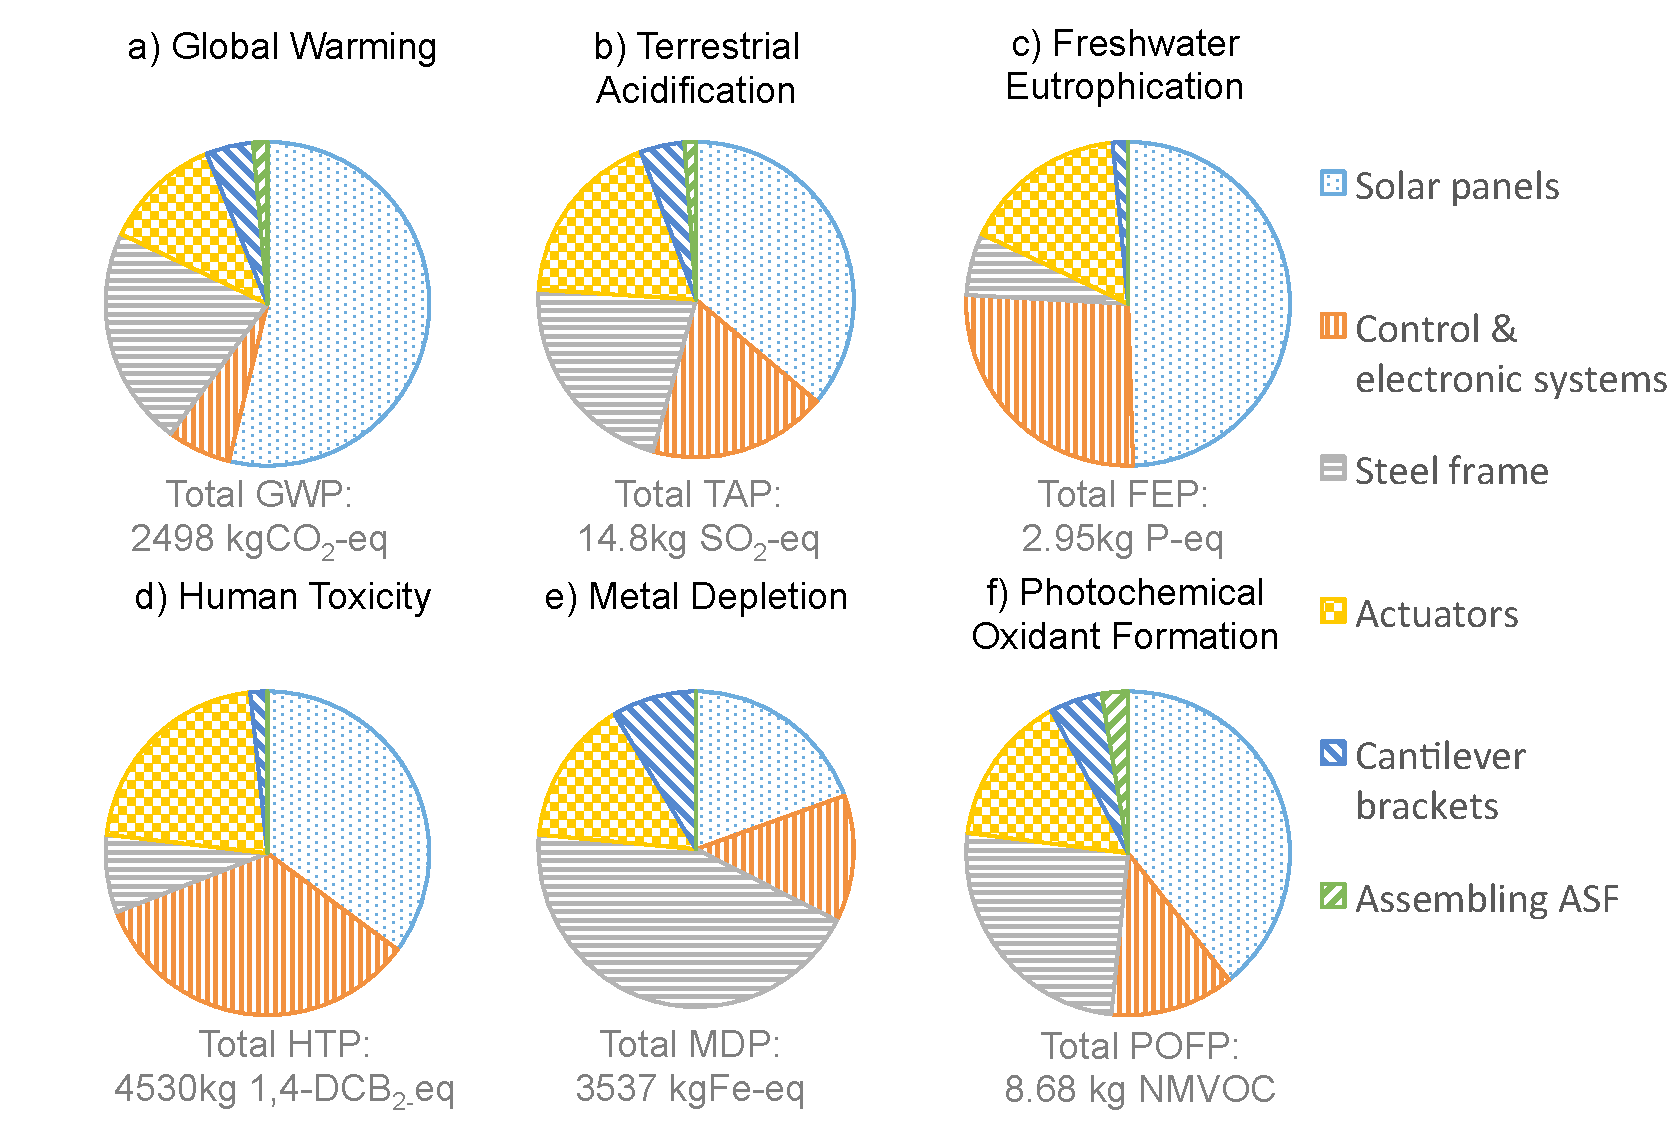
\includegraphics[width=\textwidth, trim= 0cm 0cm 0cm 0cm,clip]{pieembodied}
\caption{Embodied emission breakdown of six major midpoint indicators. The solar panels, control/electronics, and steel frame have the highest life cycle impact}
\label{fig:embodied}
\end{center}
\end{figure}

\subsection{Calculation of GWP Emission Factor}
The combined GWP of main inputs to the ASF, previously described in Figure \ref{fig:BOS}, can be illustrated using a waterfall chart as shown in Figure \ref{fig:waterfall}. 


This gives us a final emission of 3037kgCO$_2$-eq. When we include the energy savings through adaptive shading in our system expansion, the final emissions come down to -8318kgCO$_2$-eq. Dividing these values by the photovoltaic electricty production over a 20 year life time of 9175kWh, we get an emission factor of 331gCO$_2$-eq/kWh for the system without adaptive shading and -906 gCO$_2$-eq/kWh with adaptive shading.


\begin{figure}[H]
\begin{center}
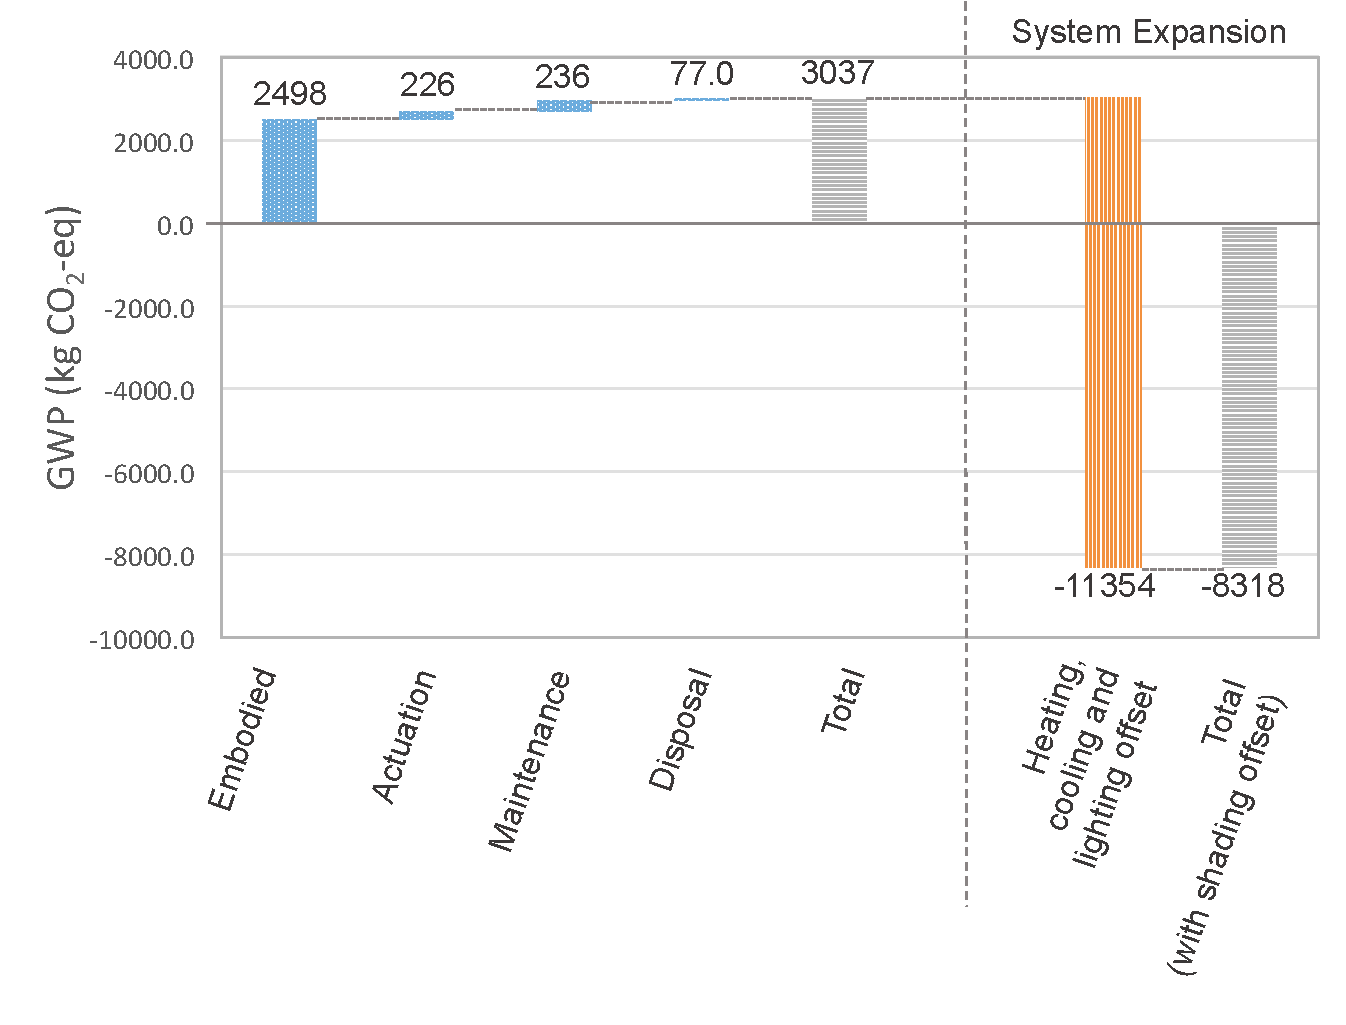
\includegraphics[width=\textwidth, trim= 0cm 0cm 0cm 0cm,clip]{waterfall}
\caption{Waterfall diagram of GWP of the ASF not including photovoltaic electricity production. When reading from left to right, the far left bar details the embodied carbon emissions. The second, third and fourth bar detail the actuation, maintenance, and disposal respectively. This leaves us with our final emissions value (grey bar) of 3037kgCO$_2$-eq. The orange bar details the emission reduction through adaptive shading which is part of our system expansion bringing the total down to -8318kgCO$_2$-eq. When we divide these totals by the photovoltaic electricity production (9174kWh) we gain an emission factor of 331gCO$_2$-eq/kWh for the system without adaptive shading and -906 gCO$_2$-eq/kWh with adaptive shading. Note that the waterfall chart itself doesn't show PV electricity generation. This is taken into account in the emission factor.}

\label{fig:waterfall}
\end{center}
\end{figure}

% \subsection{Global Distribution of GWP and Terrestrial Acidification}


% \textcolor{magenta}{\textit{Sorry that I keep coming back to this. How is this relevant to the overall scope of the paper? You should probably pick it up again in the Conclusion or Discussion. Furthermore you should describe (e.g. in the Methodology) how the regionalized LCA was performed.\\
% As I said - these figures are likely to be wrong. If one of the reviewers is an LCA crack, he / she might attack this.}}

% The global distribution of embodied GWP emissions is focused in Europe, specifically Germany and Switzerland as most of the manufacturing is done in this region. It can be see however that emissions occur globally due the sourcing of primary materials from many locations around the world. Terrestrial acidification however is more interesting as it has a local impact compared to carbon emissions. It is interesting to note that China carries the greatest burden of terrestrial acidification from the ASF production.
 
% \begin{figure}[H]
% \begin{center}
% 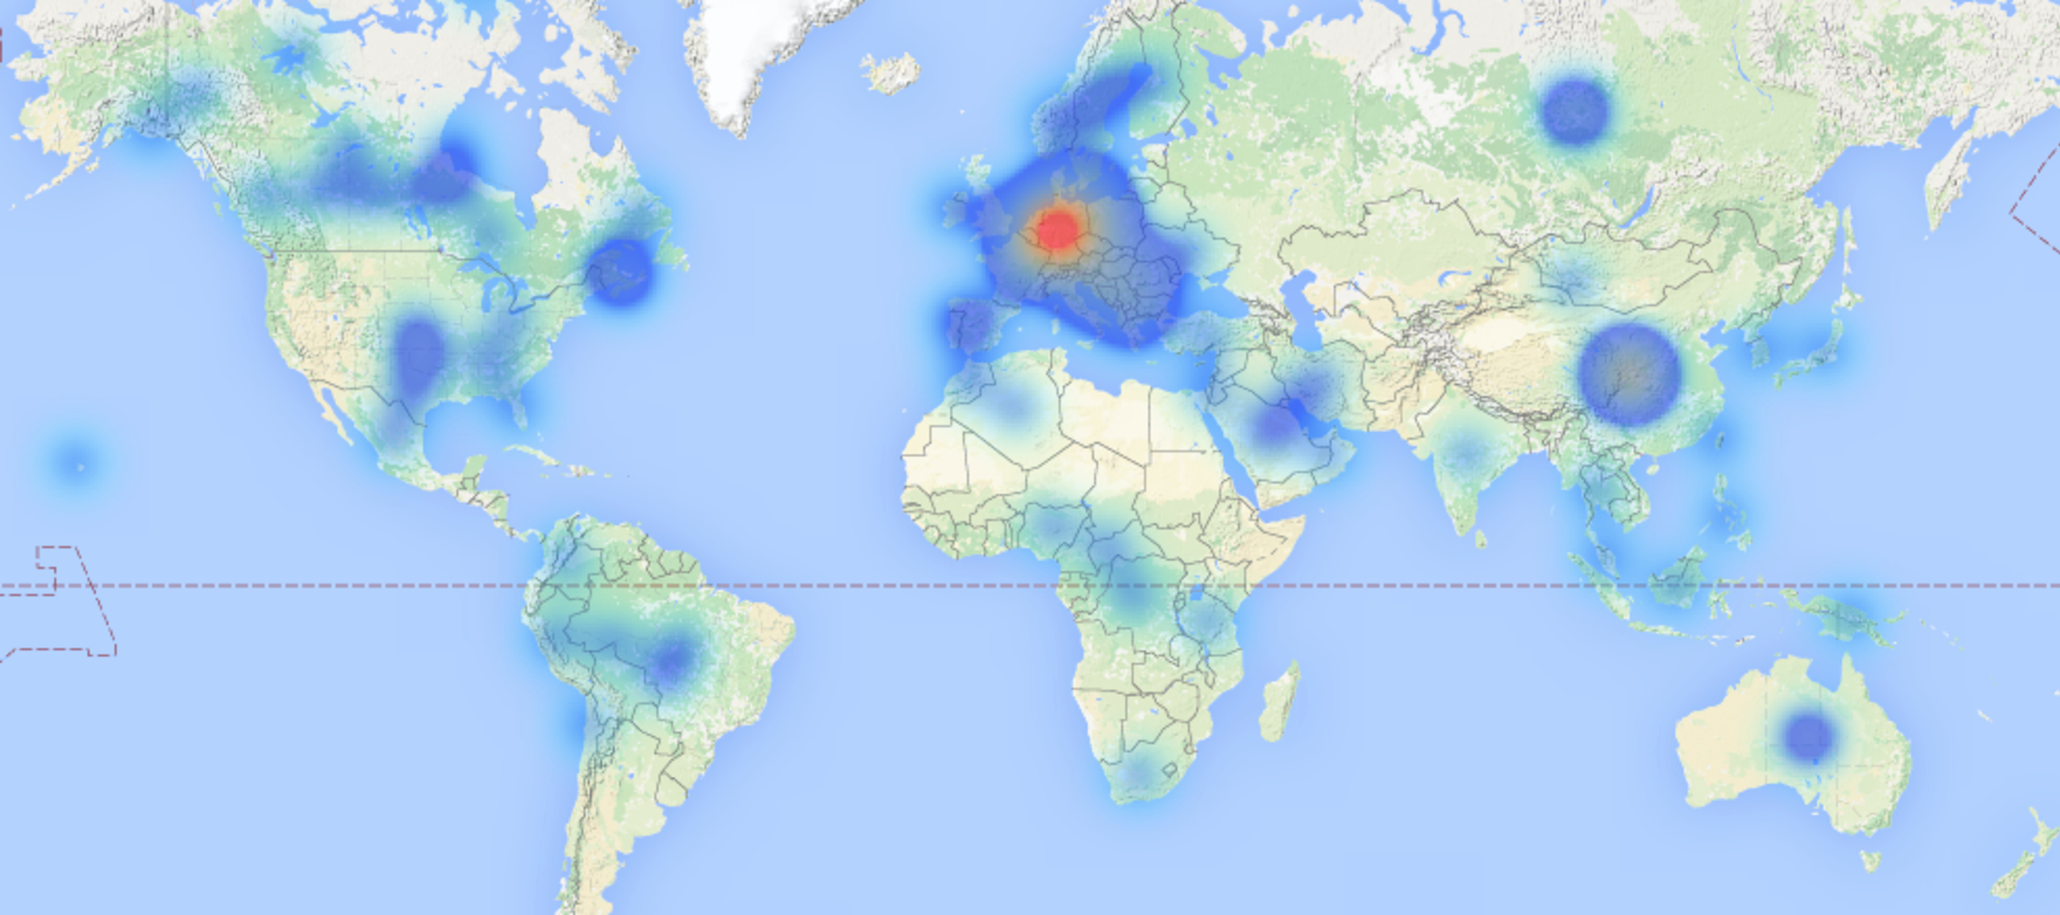
\includegraphics[width=10cm, trim= 0cm 0cm 0cm 0cm,clip]{mapGWP.pdf}
% \caption{Global distribution of embodied GWP emissions}
% \label{fig:mapGWP}
% \end{center}
% \end{figure}

% \begin{figure}[H]
% \begin{center}
% 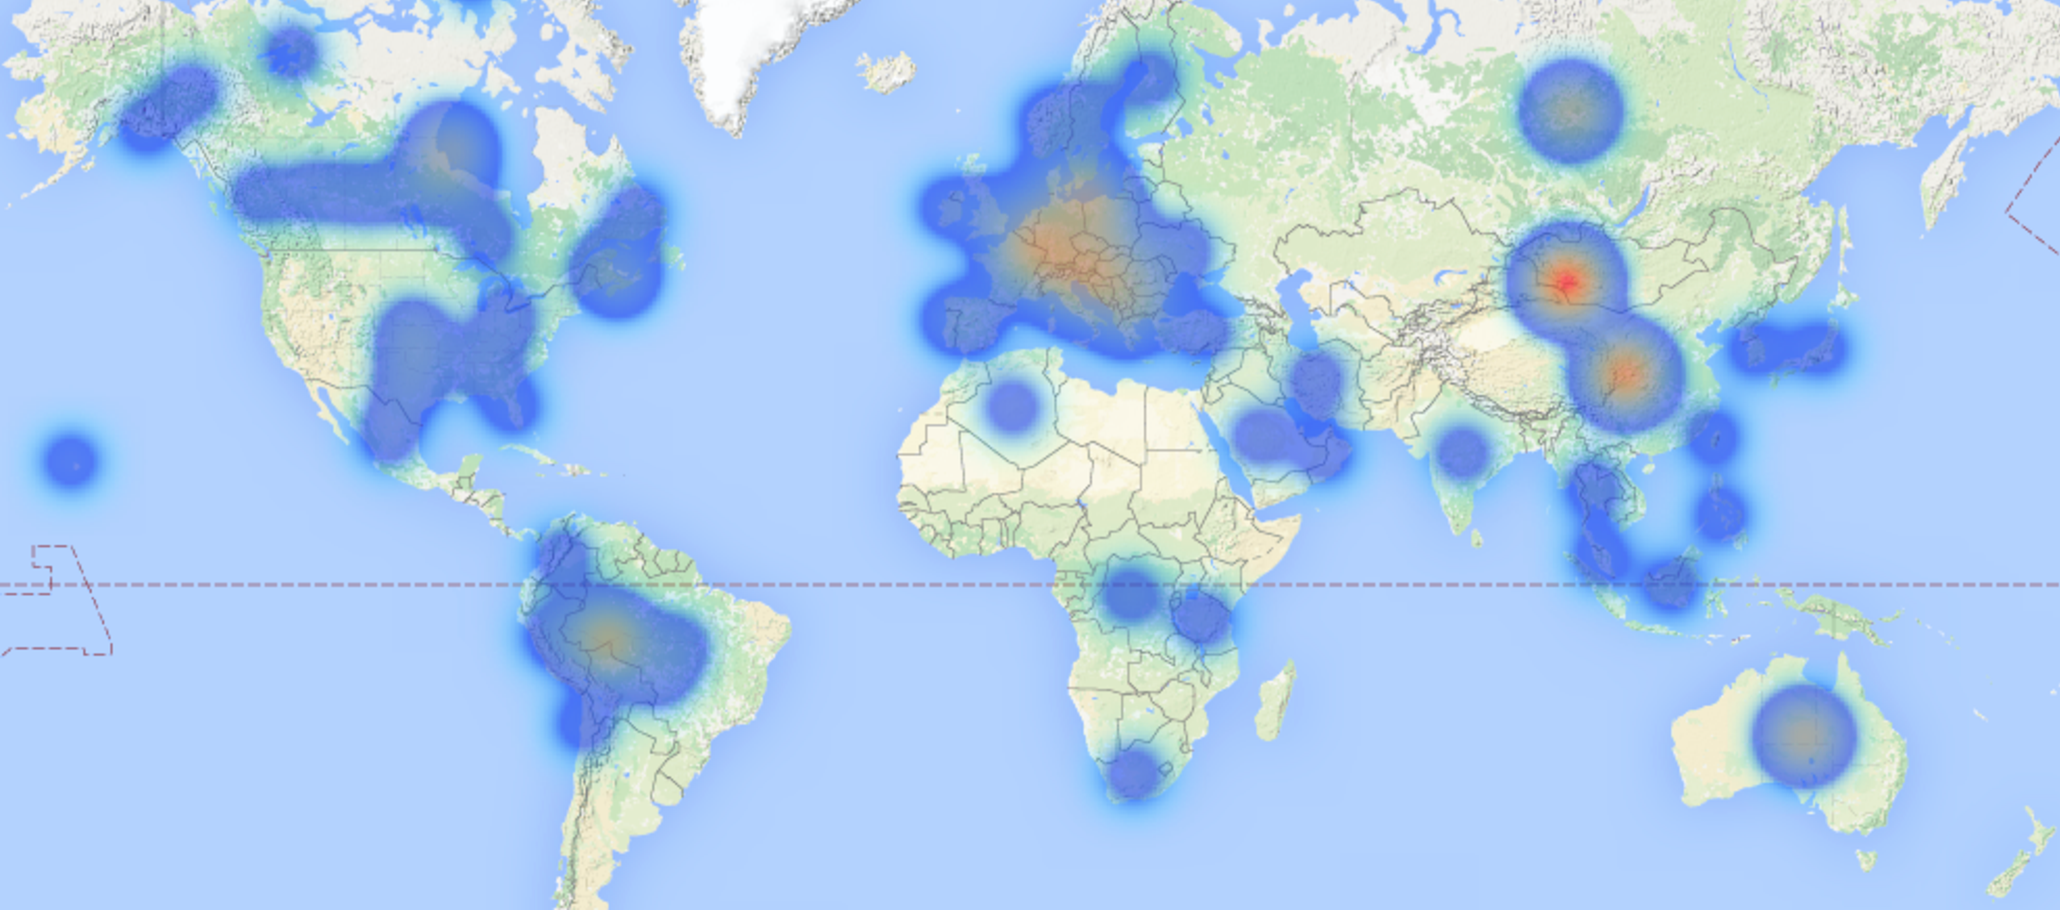
\includegraphics[width=10cm, trim= 0cm 0cm 0cm 0cm,clip]{mapacidification.pdf}
% \caption{Global distribution of terrestrial acidification}
% \label{fig:mapAcid}
% \end{center}
% \end{figure}

\subsection{Sensitivity Analysis}


The sensitivity analysis is shown in Figure \ref{fig:sens}. The performance of the ASF is dependent on the location where it is operated as explained in Section \ref{ch:Meth:Opp}. Changing the weather files of the simulation, and the electricity mix of the country brings interesting results. Geneva has a similar climate to Frankfurt, however the local electricity mix is dominated by hydro and nuclear power which has a very low GWP potential\cite{itten2012life}. This would then increase the emission factor of the ASF to 53.5 gCO$_{2}$-eq/kWh. This difference arises as the greenhouse gas emission savings of adaptive shading are dependent on the emission factor of the grid mix.
Spain on the other hand has a warmer climate, with higher solar radiation, but a less greenhouse gas intensive electricity mix. This ultimately results in a similar emission factor of the ASF of -825 gCO$_{2}$-eq/kWh.\\


We also present a case where we remove the actuators and necessary control system for a dynamic system. Instead, we have panels that are optimally orientated at 45$^{\circ}$ to the horizontal axis. This reduces embodied greenhouse gas emissions by 12.1\% from the baseline highlighted in Figure \ref{fig:embodied}. However the reduction in electricity production, and savings through adaptive shading, result in a 15\% higher emission factor.\\

The choice of actuator has a small impact on the embodied carbon emissions. Changing a single Soft Robotic Actuator (including the air compressor, tubing, and maintenance) to a classical servo motor increases the total embodied GWP by 23\% from 2498 kg CO$_{2}$-eq to 3073 kg CO$_{2}$-eq. However, the servo motors have lower operational emissions and maintenance. Ultimately an ASF with servo motors has a 1.5\% higher emission factor. \\
%\textcolor{magenta}{\textit{(Is this cited or was it also calculated? Do we provide the inventory?)}} \textcolor{red}{\textit{(Calculated, but inventory of motors needs to go in the Appendix)}}.\\

The control system design should be carefully thought out due to the high embodied human toxicity, freshwater eutrophication and terrestrial acidification. However simplifying the actuation control electronics has a minimal effect as the majority of the emissions lie in the inverter, cables, and air compressor. In terms of GWP, there is a 0.3\% difference which is insignificant.

%\textcolor{red}{The Monte Carlo Simulation did not yield any significant results / was significant. } \textcolor{blue}{Fill this out once your results come in}

% In Switzerland, we see a 6\% reduction compared to the average electricity mix. This is because the Swiss electricity mix is dominated by hydro and nuclear power which has a very low GWP potential [citation needed\textcolor{magenta}{ \textit{ecoinvent?}}]. In Germany on the other hand, the ASF has a 81\% reduction in carbon emissions as the emission factor of the electricity grid is roughly five times higher compared to Switzerland [citation needed] due to the relatively high share in coal-fired power plants.\\

\begin{figure}[H]
\begin{center}
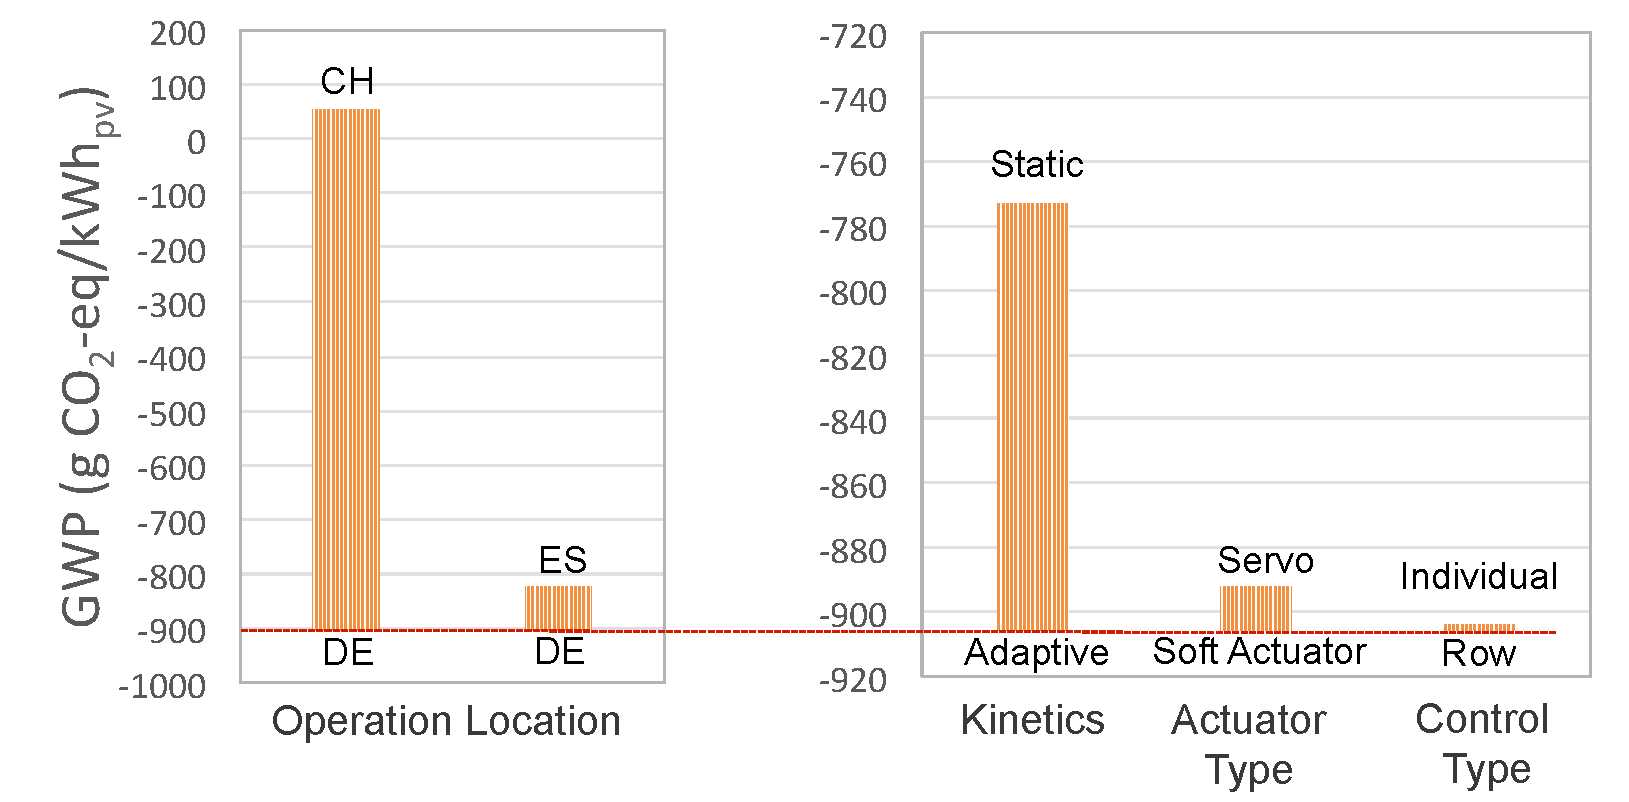
\includegraphics[width=10cm, trim= 0cm 0cm 0cm 0cm,clip]{sens.pdf}
\caption{Sensitivity analysis of the emission factor including the HVAC impact of adaptive shading based on location, actuation system, and control system}
\label{fig:sens}
\end{center}
\end{figure}

\subsection{Comparison to existing PV technologies}

Comparison of the ASF to other PV technologies and the German electricity mix is highlighted in Figure \ref{fig:compPV}. This comparison is conducted in Frankfurt am Main with an average irradiation of 855 kWh/m$2$/year.\

The blue bars detail systems with no added shading benefits. Here we present the ASF, a static optimally orientated facade as used in Figure \ref{fig:sens}, and three classical flat facade installations.  
The orange bars detail the system expansion where the ASF is built over glazed surfaces which also bring energy savings to the building. Because the GWP savings through adaptive shading offsets the entire embodied GWP, we have a system with a negative emission factor.



%Note that the just panels of the ASF, without the BOS, still has a higher emission factor than the CIGS installation. This is due to lower power production as a result of self shading \cite{hofer2015photovoltaics}, and situations where the panels are not optimally positioned\textcolor{magenta}{\textit{Where do these GHG figures come from?}}.



\begin{figure}[H]
\begin{center}
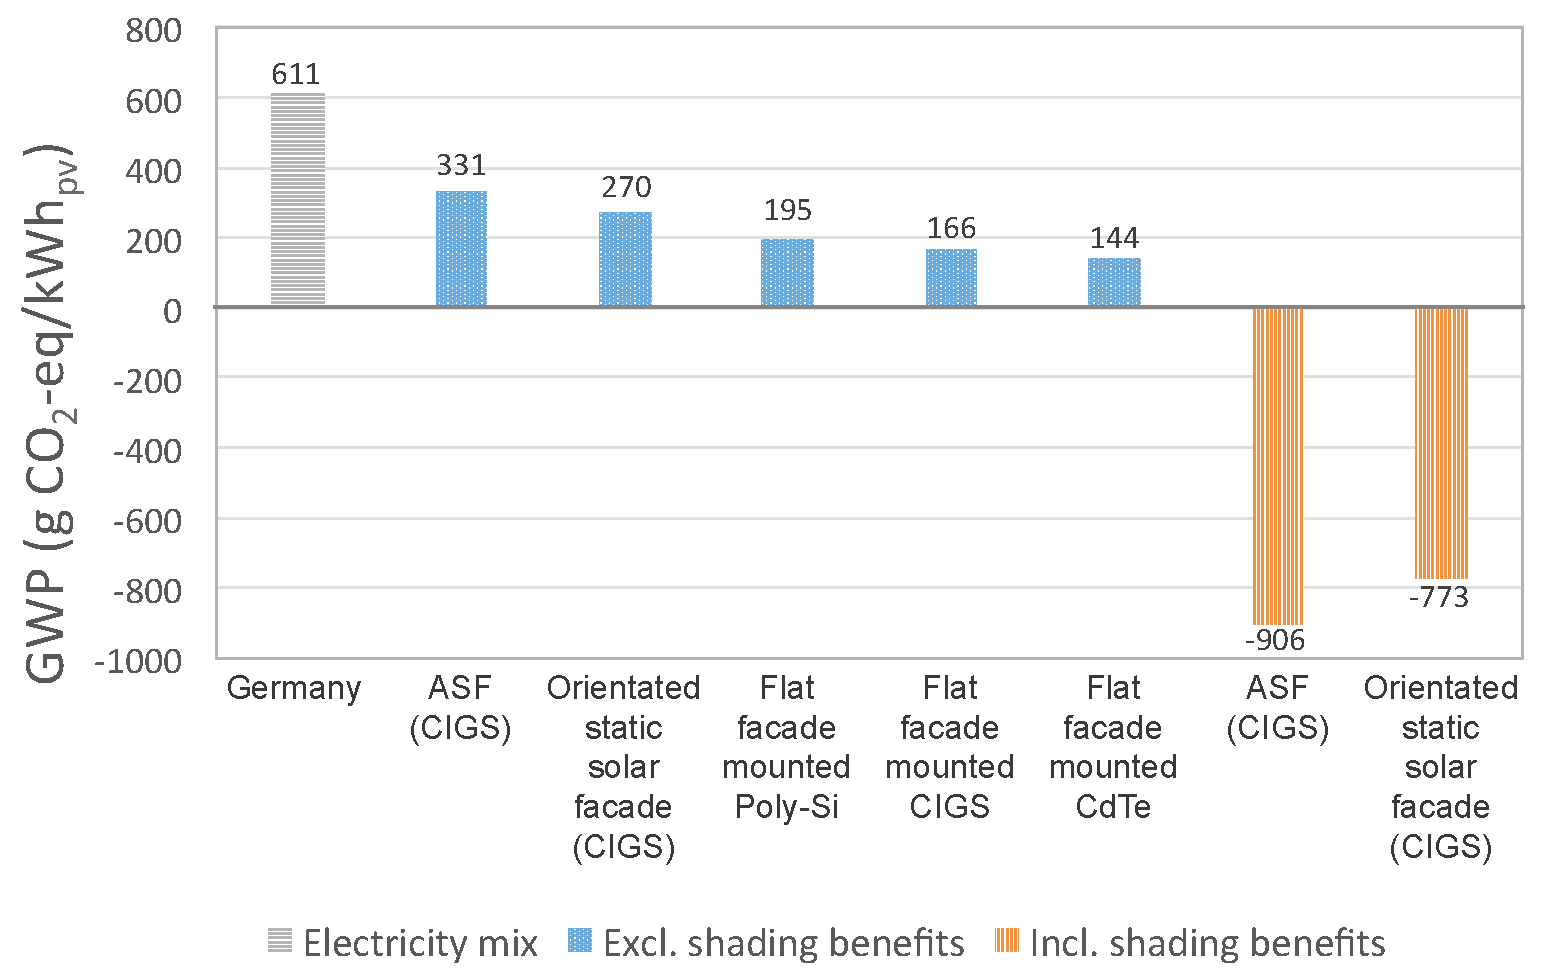
\includegraphics[width=10cm, trim= 0cm 0cm 0cm 0cm,clip]{compPV.pdf}
\caption{Comparison of facade installations in Germany with an average facade irradiation of 855kWh/m2/year.
We compare an ASF to an optimally orientated static facade, and classic flat facade mounted PV solutions. The orange bars include the system expansion of energy savings through adaptive shading.}
\label{fig:compPV}
\end{center}
\end{figure}




\section{Discussion}
\label{ch:discussion}
\input{5_discussion}

\section{Conclusion}
\label{ch:conclusion}
% !TEX root = main.tex

The environmental performance of the ASF has been shown to be favorably competitive with a classic BIPV installation. Even though the embodied environmental performance is \textcolor{red}{six times} worse than a static CIGS installation, it is offset three fold through adaptive shading. This combination of adaptive shading with photovoltaic generation brings new advantages to solar as it effectively has a negative emission factor of \textcolor{red}{-470.1 g CO2/kWh}. These advantages however, will not be present if the ASF is installed over an opaque building surface. It is therefore better to install static systems over opaque facades, and keep the adaptive system for glazed facades only. \\

The design of an ASF naturally can greatly influence the results. Varying factors such as the choice of actuators and the complexity of the control system can change the emission factor. The largest variable however is the emission factor of the grid electricity mix. The building operational savings in heating, cooling, and lighting will have a CO2 saving based on the grid electricity mix. A country with low CO2 grid mix, such as Switzerland, will have an emission factor of \textcolor{red}{140gCO2/kWh}. In Germany on the other hand, will have an emisison factor of \textcolor{red}{-700gCO2/kWh}.\\

Future research will validate the numerical simulations experimentaly. This will be conducted on the ETH House of Natural Ressources (http://www.honr.ethz.ch) living lab where an example of an ASF has already been constructed \cite{nagy2015frontiers}. Further numerical simulations of the ASF on different building typologies, building systems and climates will enable us to specifically target the best application scenario. An application of the ASF in Spain for example could yield even larger energy savings compared to a temperate climate like Switzerland.\\

To conclude, we demonstrated that BIPV systems and adaptive shading elements complement each other successfully. We see an improvement in environmental performance of the PV technology, and create new architectural possibilities for the aesthetic integration of PV panels over glazed building surfaces. 

%The END


% The use of soft robotic actuators over servo motors increases the environnmental performance by \textcolor{red}{60 kgCO2} per square meter. The control electronics, which represents 11\% of the total embodied emissions, can increase by \textcolor{red}{35\%} if we increase the resolution of the facade so each panel can move independently. Also the supporting structure, representing \textcolor{red}{20\%} of total emissions can be better optimised to use less steel, or an alternative material. \\

\section{Acknowledgments}
\label{ch:acknowledgments}
% !TEX root = main.tex

The authors would like to acknowledge the HiLo and HoNR project members for the design and construction of the ASF: Supermanoeuvre (Sydney Australia) and the Professorship of Architecture and Structures (BRG, ETH Zurich) for their work in designing the HiLo building; and the Institute of Structural Engineering (IBK, ETH Zurich) for their work in designing the HoNR building. We would also like to thank Stefanie Hellweg for her support in the LCA analysis. The authors would also like to thank other key contributors to the ASF Project: Bratislav Svetozarevic, Moritz Begle, Johannes Hofer, Nicola Offeddu, and Giovanni Bianchi. \\

This research was partly funded by the Climate-KIC, Building Technologies Accelerator program.


\section{Appendix}
\label{ch:appendix}
% !TEX root = main.tex





%% appendix sections are then done as normal sections
%% \appendix
%% \section{}
%% \label{}

%% bibitems, please use
  \bibliographystyle{elsarticle-num} 
  \bibliography{references}

\end{document}
\endinput